\documentclass[11pt]{article}

\usepackage[style=script-v2, privacy=anonym]{../tools/library}

\newcommand{\book}{[Riehl, E.: Category Theory in Context] }

\renewcommand{\Lecturer}{Prof. U. Krähmer}

\begin{document}
\head{Category Theory}{Part II.2: Universal Properties and the Category of Elements}

\tableofcontents

\newpage
\section{Introduction}
Wir erinnern uns zurück...
\begin{definition} \Xlabel{Definition}{subsub}{Darstellbare Funktoren}
    Sei $C \in \Cat$, lokal klein. Ein ko- (bzw. kontra-) varianter Funktor $F: C \to \Set$ heißt \emph{darstellbar}, falls 
    \begin{enumerate}[label=(\roman*)]
        \item ein natürlicher Isomorphismus $\alpha: C(c,-)\overset{\cong}{\Longrightarrow}F$ zwischen dem Hom-Funktor $C(c,-)$ und $F$ im kovarianten Fall oder
        \item ein natürlicher Isomorphismus $\beta: C(-,c)\overset{\cong}{\Longrightarrow} F$ zwischen dem Hom-Funktor $C(-,c)$ und $F$ im kontravarianten Fall 
    \end{enumerate}
    für ein Objekt $c\in \Ob(C)$ existiert.
\end{definition}

\begin{note}[zu Definition \ref{Darstellbare Funktoren}]\mbox{}
\begin{enumerate}[label=-]
    \item Ein beliebiger kovarianter Funktor $F:C\to \Set$ mit Domain lokal klein schickt ein Objekt $c$ auf eine Menge $Fc$ und einen Morphismus $f:c\to d$ auf eine Mengenabbildung $Ff: Fc \to Fd$.
    \item Falls $F$ durch ein $c$ darstellbar sein sollte, dann können wir jede beliebige Zielmenge $Fd$ eines Objektes $d\in C$ gerade identifizieren mit der \emph{Menge der Morphismen} $C(c,d)$ von $c\to d$ (starke Aussage über Kardinalität usw...); und gleichzeitig jeden Zielmorphismus $Ff: Fd\to Fe$ mit der \emph{Präkomposition} $f^*: C(c,d) \to C(c,e), g\mapsto f\circ g$ (und da kann es sein, dass einige Objekte zusammenfallen, nicht alles getroffen wird, usw... ABER: es gibt eine exakte Identifikation)
\end{enumerate}
\end{note}

Letztes Mal haben wir uns über die Existenz solcher Darstellbarkeiten Gedanken gemacht und dabei eines der wichtigsten Sätze der Kategorientheorie festgehalten:

\begin{theorem} \Xlabel{Satz}{subsub}{Yoneda-Lemma, Kovarianter Fall} Für jeden kovarianten Funktor $F:C \to \Set$ aus einer lokal kleinen Kategorie $C$ ist die folgende Abbildung eine Bijektion:
$$\Hom{C(c,-)}{F}\longrightarrow Fc$$
$$\alpha \longmapsto \alpha_c(\id_c)$$
\end{theorem}

\begin{note}[zu Satz \ref{Yoneda-Lemma, Kovarianter Fall}] Versuchen wir noch mal kurz nur ansatzweise die bedeutende Tragweite dieses Satzes zu verstehen.
\begin{enumerate}[label=-]
    \item Der Satz liefert eben nicht nur überhaupt eine Existenz von natürlichen Transformationen für jeden beliebigen Funktor $F$ aus einer lokal kleinen Kategorie, sondern sogar genau die Anzahl solcher $\alpha: C(c,-)\Longrightarrow F$ für jedes $c\in \Ob(C)$. Mit anderen Worten:
    \begin{quote}
        ''Für jedes Objekt $c\in \Ob(C)$ gibt genau so viele natürliche Transformationen $\alpha: C(c,-)\Longrightarrow F$, wie es Elemente in $Fc$ gibt.''
    \end{quote}
    \item Im Beweis zeigen wir diese Bijektion mittels Umkehrabbildung, doch eine viel bessere Intuition wird in Beispiel 2.2.1 in Riehls Buch vermittelt; nämlich die Transformation aus der Ordinalen Kategorie $\bbomega$ nach $F$. Aus dieser Überlegung ging hervor, dass jede natürliche Transformation \emph{wegen ihrer Natürlichkeit} eindeutig durch Bild von $\alpha_k(\bbomega(k,k))$, also das Bild eines Singletons $*$ bestimmt ist.
    Dies gleicht der Auswahl eines Elements aus $Fk$...
    \item[\textbf{!}] Im Allgemeinen sind die Transformationen $\alpha\in \Hom{C(c,-)}{F}$ keine Isomorphien. Daher wissen wir nicht genau, ob $F$ auch tatsächlich immer darstellbar ist, bzw. gibt es in der Tat Funktoren, die \emph{nicht darstellbar} sind.
\end{enumerate}
\end{note}

Heute wollen wir studieren, wie die Hom-Funktoren $C(c,-)$ konkret bezüglich des Objektes $c\in \Ob(C)$ aussehen können. Gibt es beispielsweise Objekte, in denen die Yoneda-Transformation besonders ''schön'' ist? Oder anders gibt es Objekte $c$ in denen die Darstellungen von $F$ sehr schön sind...?
Insbesondere beantworten wir die Fragen, die Riehl am Ende von Kapitel §2.1 stellt.

\newpage

\section{Universal Properties and Universal Elements}

\subsection{Motivation}
\begin{definition} \Xlabel{Definition}{subsub}{Konstanter Funktor}
Sei $C$ eine lokal kleine Kategorie. Der konstante Funktor $\Delta*$ ist definiert durch:
$$ \Delta*: \quad C\longrightarrow \Set, \quad \Ob(C)\ni c\longmapsto *,\quad C(c,d)\ni f \longmapsto \id_*$$
    
\end{definition}
\begin{definition} \Xlabel{Definition}{subsub}{Initiale und Terminale Objekte}
    Sei $C$ eine lokal kleine Kategorie. Ein Objekt $c\in \Ob(C)$ heißt 
    \begin{enumerate}[label=(\roman*)]
        \item \emph{initial}, falls der Hom-Funktor $C(c,-): C\to \Set$ natürlich isomorph zum konstanten Funktor $\Delta*: C\to \Set$ ist
        \item \emph{terminal}, falls der Hom-Funktor $C(-,c): C\op \to \Set$ natürlich isomorph zum konstanten Funktor $\Delta*: C\op\to \Set$
    \end{enumerate}
\end{definition}

Mit der Terminologie die uns bereits zur Darstellbarkeit zur Verfügung steht, folgt tautologisch:

\begin{corollary}[Äquivalenz Darstellbarkeit und Existenz initialer / terminaler Objekte]
    Eine Kategorie $C$ besitzt genau dann ein initiales (bzw. terminales) Objekt, wenn der Funktor $\Delta*: C\to \Set$ (bzw. $\Delta*: C\op \to \Set$) darstellbar ist.
\end{corollary}

\begin{definition} \Xlabel{Definition}{subsub}{Universelle Eigenschaft}
    Sei $F: C\to \Set$ ein darstellbarer Funktor und $F\cong C(c,-)$. Dann sagen wir:
    \begin{quote}
        $F\cong C(c,-):\Longleftrightarrow$ ''$F$ codiert die universelle Eigenschaft von $c$.''
    \end{quote}
\end{definition}

\begin{note}[zu Definition \ref{Initiale und Terminale Objekte}, \ref{Universelle Eigenschaft}]\mbox{}
    \begin{enumerate}[label=-]
        \item Die Definition \ref{Universelle Eigenschaft} soll unsere Definition \ref{Initiale und Terminale Objekte} erweitern, in dem Sinne, dass es noch mehr universelle Eigenschaften gibt, als ''initial'' und ''terminal''. 
        \item Wir bezeichnen für kovariante darstellbare Funktoren, dass $c$ eine ''\emph{mapping-out}'' universelle Eigenschaft besitzt und vice versa für kontravariante Funktoren: $c$ besitzt eine ''\emph{mapping-in}'' universelle Eigenschaft.
    \end{enumerate}
\end{note}

\newpage
\begin{note} \label{questions} Es kommen natürliche Fragen auf (vgl. §2.1):
\begin{enumerate}
    \item Wie einzigartig sind diese universellen Eigenschaften? Genauer: Falls zwei Objekte $c$ und $c'$ denselben Funktor darstellen, sind diese dann (natürlich) isomorph?
    \item Welche Informationen werden zur Konstruktion eines natürlichen Isomorphismus zwischen dem darstellbaren Funktor $F$ und seiner Darstellung $C(c,-)$ benötigt?
    \item Wie hängen universelle Eigenschaften dargestellt durch Funktoren mit initialen und terminalen Objekten zusammen?
\end{enumerate}
\end{note}

\subsection{Zentrale Resultate}

\begin{theorem} \Xlabel{Satz}{subsub}{Äquivalenz kategorielle und darstellende Isomorphie}. Sei $C$ eine lokal kleine Kategorie. Dann sind die folgenden Aussagen für $x,y\in \Ob(C)$ äquivalent bzw. enthalten dieselben Informationen:
\begin{enumerate}[label=(\roman*)]
    \item $x\cong y$ in der Kategorie $C$.
    \item $C(-,x)\cong C(-,y)$ in der Kategorie $\Set^{C\op}$
    \item $C(x,-)\cong C(y,-)$ in der Kategorie $\Set^C$
    \end{enumerate}

\begin{proof} Die Äquivalenzen (i) $\Leftrightarrow$ (ii) sowie (i) $\Leftrightarrow$ (iii) folgen aus direkt als Konsequenz aus der volltreuen Eigenschaft der Yoneda Einbettungen $\yoneda: C\hookrightarrow \Set^{C\op}$ und $\yoneda: C\op \hookrightarrow \Set^C$. Wir rechnen zur Übung das ganze noch einmal nach, um die Aussagen ''Funktoren erhalten Isomorphismen'' (Lemma 1.3.8) und ''volltreue Funktoren reflektieren Isomorphismen'' (Übung 1.5.iv) zu verinnerlichen.\bigskip

(i) $\Longrightarrow$ (ii): Sei $f:x\to y \in C(x,y)$ ein Isomorphismus. Dann existiert ein beidseitig inverser Morphismus $g:y\to x$ mit $f\circ g = \id_y$ und $g\circ f = \id_x$. Betrachte noch einmal präzise die Yoneda-Einbettung $\yoneda: C\hookrightarrow \Set^{C\op}$\bigskip

Für Objekte $x\in \Ob(C)$\bigskip

$\displaystyle \yoneda(x) = \ C(-,x): \begin{cases} 
    c\mapsto C(c,x) \\
    [g: c \to c'] \mapsto [g^*: C(c',x) \to C(c,x),\ h\mapsto h\circ g]
\end{cases}$\bigskip

$ \displaystyle \mbox{}\hspace{1cm}  = C(-,x): C\op \to \Set $ ... kontravarianter Funktor \bigskip 

Für Morphismen $f\in C(x,y)$\bigskip

$\displaystyle \yoneda(f) = f_*:  \begin{cases}
    C(c,x)\ni h\mapsto f\circ h \in C(c,y) \text{ auf den Objekten in $\Set$}\\
    [g^*:C(c',x) \to C(c,x),...] \mapsto [f\circ g^*: C(c',y) \to C(c,y),...]\\
    \text{ auf den Morphismen in $\Set$}
\end{cases}$\bigskip

$\displaystyle = f_*: C(-,x) \Longrightarrow C(-,y)$ ... natürliche Transformation zwischen Funktoren\bigskip

Dann wäre zu überprüfen, ob $\yoneda(g) \circ \yoneda(f) = \id_{C(-,x)}$ und $\yoneda(f)\circ \yoneda(g) = \id_{C(-,y)}$
Und tatsächlich, seien $c\in \Ob(C)$ und $h\in C(c,x)$ beliebig.
$$(\yoneda(g)\circ \yoneda(f))(h) = g_*\circ f_*(h) = g\circ (f\circ h) = (g\circ f)\circ h = id_x \circ h = h$$
hier bereits $\yoneda(g) \circ \yoneda(f)|_{\Ob(\Set)} = \id_{\Ob(\Set)}$.
Seien nun noch $c,c'\in \Ob(C)$ und $i^*: C(c,x) \to C(c',y)$ und $h\in C(c,x)$ beliebig. Dann ist
$$(\yoneda(g)\circ \yoneda(f))(i^*(h)) = g_*\circ f_*(i^*(h)) = g\circ (f\circ (h\circ i)) $$
$$= (g\circ f)\circ (h\circ i) = (id_x \circ  h) \circ i =  h\circ i = i^*(h)$$
Also auch $\yoneda(g)\circ \yoneda(f)|_{\hom(\Set)} = \id_{\hom(\Set)}$ und für Rechtsinversion simultan. \bigskip

(ii) $\Longrightarrow$ (i): Sei $\alpha: C(-,x) \Longrightarrow C(-,y)$ ein natürlicher Isomorphismus zwischen Funktoren. Es gilt zu zeigen, dass dann auch $x\cong y$ in $C$. \bigskip

Da $\yoneda: C \to \Set^{C\op}$ voll ist, gibt es einen Morphismus $f\in C(x,y)$ mit $\yoneda(f) = \alpha$ sowie einen Morphismus $g\in C(y,x)$ mit $\yoneda(g) = \alpha\r$. Nun ist allerdings leicht zu sehen, dass 
$$\yoneda(g\circ f) = (g\circ f)_* (\cdot) = (g\circ f)\circ(\cdot) = g\circ(f\circ(\cdot))= g_*(f_*(\cdot))=(\alpha\r\circ\alpha)(\cdot)= \id_{C(-,x)}$$
Und andersherum genauso. Da $\yoneda$ ebenfalls treu ist, folgt aus $\yoneda(g\circ f) = \id_{C(-,x)}$ bereits $g\circ f = \id_x$.\bigskip

Aus Dualitätsgründen gilt auch (i) $\Longleftrightarrow$ (iii). 
\end{proof}
\end{theorem}

\begin{corollary}
    Seien $x,y\in \Ob(C)$ und stellen denselben Mengen-wertigen Funktor dar. Dann sind $x$ und $y$ isomorph, mehr noch: Es gibt einen eindeutigen Isomorphismus $f: x\to y$ der mit allen natürlichen Transformationen kommutiert.
\end{corollary}

\begin{corollary}
    Die Unterkategorie einer Kategorie $C$ aufgespannt durch ihre terminalen Objekte ist entweder leer oder ein kontrahierbarer Gruppoid, gemeint natürlich isomorph zur terminalen Kategorie $\1$.
\end{corollary}

\begin{definition} \Xlabel{Definition}{subsub}{(Universelles) Element}
    Ein \emph{Element} eines ko- (bzw. kontra-) varianten, mengenwertigen Funktors $F$ induziert durch die Kategorie $C$ ist ein Objekt $c$ zusammen mit einem Element $x\in Fc$. Ein Element heißt \emph{universell}, falls die natürliche Transformation $\alpha_x : C(c,-)\Longrightarrow F$ aus dem Yoneda-Lemma mit $\alpha_x(\id_c) = x$ ein natürlicher Isomorphismus ist. In diesem Fall stellt $c$ $F$ dar und $\alpha_x$ definiert eine Darstellung für $F$.
\end{definition}

\begin{note}[zu Definition \ref{(Universelles) Element}]
    \mbox{}
    \begin{enumerate}[label=-]
        \item Im Unterschied zu Definition \ref{Darstellbare Funktoren} stellt das universelle Element stark konstruktive (und wie wir später feststellen werden / oder in Kapitel §2.2 bereits festgestellt haben, alle wesentlichen) Informationen über den dargestellten Funktor $F$ bereit.
    \end{enumerate}
\end{note}
\subsection{Konklusion}
Wir wollen noch einmal explizit die Fragen gestellt in Bemerkung \ref{questions} beantworten:
\begin{note}[zu Bemerkung \ref{questions}]\label{answers}\mbox{}
\begin{enumerate}[label = zu \arabic*.:]
    \item Stellen zwei Objekte denselben Funktor $F$ dar, so sind sie eindeutig isomorph zueinander. Jeder darstellbare Funktor $F:C\to \Set$ ist also eindeutig dargestellt bis auf Isomorphie.
    \item Bereits beantwortet in §2.2 Yoneda Lemma, nämlich ein einziges Objekt in $Fc$
    \item Eine abschließende Antwort liefert der letzte Teil des Vortrags, und die lautet: Sie sind dieselbe Sache, nur in einer anderen Kategorie. Korollar 2.4 hat bereits erkannt, dass initial und terminal Spezialfälle einer Äquivalenz von Darstellbarkeit sind. Gilt auch die Umkehrung? 
\end{enumerate}
\end{note}

\newpage
\subsection{Beispiele}
\begin{example} \Xlabel{Beispiel}{subsub}{Vergissfunktor I}
    Der Vergissfunktor $U: \Ring \to \Set$ wird dargestellt durch das universelle Element $\Z[x]$ mit $x\in \Z[x]$. $$\Ring(\Z[x], R) \cong UR$$
\end{example}

\begin{example} \Xlabel{Beispiel}{subsub}{G-Torsor} Sei $E: \mathrm B G \to \Set$ ein Funktor, zum Beispiel eine linke $G$-Menge / eine Linkswirkung $E\curvearrowright X$. $E$ ist genau dann darstellbar, wenn es einen Isomorphismus $G\cong E$ von linken $G$-Mengen gibt. Das heißt $E$ ist
\begin{enumerate}
    \item frei. $\Stab(x) = \{\1\}$ für alle $x\in E$
    \item transitiv. $\mathrm{Orb}(x) = G$ für alle $x\in E$
    \item nichtleer. $E \neq \leer$
\end{enumerate}
Umgekehrt ist jede nicht-leere transitive und freie linke G-Menge isomorph zu G. Nach dem Yoneda Lemma ist ein Isomorphismus $G\cong E$ bestimmt durch die Wahl eines Elements $e\in E$ als Bild von $e\in G$ unter der natürlichen Isomorphie. So gesprochen, ist eine darstellbare linke $G$-Menge $E$ eine Gruppe, die ihr neutrales Element vergessen hat. Wir nennen so etwas einen $G$-Torsor. Wir haben beispielsweise $\mathbb A^n \cong \R^n$, der $n$-dim. affine Raum, der anschaulich ein $\R^n$ ohne Ursprung $o$ ist.
\end{example}

\begin{example}\Xlabel{Beispiel}{subsub}{Tensorprodukt}
Seien $V,W$ fixe $\K$-Vektorräume. Dann betrachte man den Funktor:
$$\mathrm{Bilin}(V,W; -): \Vect_\K \to \Set$$
der jedem Vektorraum $U\in \Ob(\Vect_\K )$ seine bilinearen Abbildungen $V\times W\to U$ zuordnet (und jedem [Vektorraum-Homo-]Morphismus $f$ seine Postkomposition $f_*$) Dieser Funktor wird repräsentiert, wer hätte es gedacht, von dem folgenden ausgezeichneten Vektorraum: $V\otimes_\K W$, dem Tensorprodukt von $V$ und $W$. Seine Definition IST auch gleich der folgende (in U) natürliche Isomorphismus:
$$\Vect_\K( V\otimes_\K W, U) \cong \mathrm{Bilin}(V,W;U)$$
Nach dem Yoneda-Lemma ist dieser natürliche Isomorphismus bestimmt durch ein universelles Element aus $\mathrm{Bilin}(V,W;V\otimes_\K W)$, also einer bilinearen Abbildung - wir nennen sie $\otimes: V\times W \to V\otimes_\K W$. Damit ist das Tensorprodukt nichts anderes als der \emph{universelle Vektorraum} ausgerüstet mit einer \emph{bilinearen Abbildung aus $V\times W$} heraus. Auch hier hilft das Yoneda-Lemma wieder dabei, das ganze zu entwirren. Dieser natürliche Isomorphismus identifiziert jegliche bilineare Abbildung $f: V\times W\to U \in \mathrm{Bilin}(V,W;U)$ mit einer linearen Abbildung $\hat{f}: V\otimes_\K W \to U$. Dazu betrachte man das Naturalitätsquadrat:

\begin{figure}[h]
    \centering
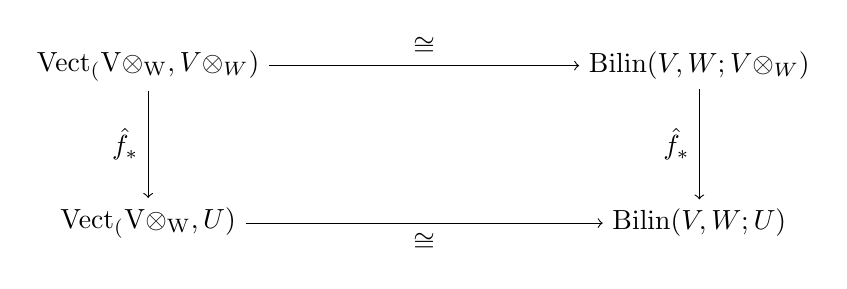
\begin{tikzpicture}
    \node (A) at (0,0) {$\mathrm{Vect_\K(V\otimes_\K W}, V\otimes_\K W)$};
    \node (B) at (7,0) {$\mathrm{Bilin}(V,W;V\otimes_\K W)$};
    \node (C) at (0,-2) {$\mathrm{Vect_\K(V\otimes_\K W}, U)$};
    \node (D) at (7,-2) {$\mathrm{Bilin}(V,W;U)$};
    
    \draw[->] (A)--(B) node[midway, above] {$\cong$};
    \draw[->] (C)--(D) node[midway, below] {$\cong$};
    \draw[->] (A)--(C) node[midway, left] {$\hat{f}_*$};
    \draw[->] (B)--(D) node[midway, left] {$\hat{f}_*$};
    
\end{tikzpicture}
\end{figure}

Verfolgt man $\id_{V\otimes_\K W}$ entlang dieses Diagramms bemerkt man, dass sich die ursprüngliche bilineare Abbildung $f$ faktorisiert durch das folgende uns schon wohlbekannte Diagramm:

\begin{figure}[h]
    \centering
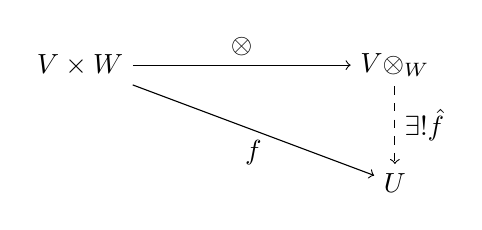
\begin{tikzpicture}
    \node (A) at (0,0) {$V\times W$};
    \node (B) at (4,0) {$V\otimes_\K W$};
    \node (D) at (4,-1.5) {$U$};
    
    \draw[->] (A)--(B) node[midway, above] {$\otimes$};
    \draw[->] (A)--(D) node[midway, below] {$f$};
    \draw[->, dashed] (B)--(D) node[midway, right] {$\exists! \hat{f}$};
    
\end{tikzpicture}
\end{figure}
\end{example}

\begin{note}[zu Beispiel 2.16] \mbox{}
    \begin{enumerate}[label=-]
        \item Jede bilineare Abbildung von $V\times W\to U$ ist eine lineare Abbildung $\hat{f}$ präkomponiert mit der universellen bilinearen Abbildung $\otimes$. Das sagt uns, dass $\otimes$ in einer bestimmten Kategorie (die wir gleich kennenlernen werden) \emph{initial} ist.
        \item Mithilfe dieser universellen Eigenschaft können wir ebenfalls die konstruktive Definition beweisen, die wir für $V\otimes_\K W$ haben. Man beachte hierzu nur, dass die Isomorphie $V\otimes_\K W \cong \Span{v\otimes w}_{v\in V, w\in W}=\im \otimes$ zu beweisen ist (Betrachte die Quotienten-Abbildung...)
    \end{enumerate}
\end{note}

Die Natürlichkeit dieser Isomorphie erlaubt es, sehr nützliche Beziehungen zu beweisen, ohne konkrete Basen zu wählen.
\begin{lemma}
Für jedes Paar an $\K$-Vektorräumen $V,W$ gilt $$V\otimes_\K W\cong W\otimes_\K V$$
\end{lemma}
\begin{proof}
    Übung. (Lösung: Zeige $$\mathrm{Bilin}(V,W;U) \overset\cong\longrightarrow\mathrm{Bilin}(W,V;U), f\mapsto f\#$$ mit $f\#(w,v):= f(v,w)$ ist ein natürlicher Isomorphismus. Komposition mit den natürlichen Isomorphismen aus Beispiel 2.16 ergibt 
    $$\mathrm{Vect_\K(V\otimes_\K W}, -)\cong \mathrm{Bilin}(V,W;-) \cong\mathrm{Bilin}(W,V;-)\cong \mathrm{Vect_\K(W\otimes_\K V}, -)$$
    und nach Korollar 2.10 muss dieser natürliche Isomorphismus zwischen Funktoren aus einer eindeutigen Isomorphie in der Ursprungskategorie $\Vect_\K $ kommen. Also $V\otimes_\K W \cong W\otimes_\K V$)
\end{proof}

\newpage
\section{The Category of Elements}
\subsection{Motivation}
Was uns bis jetzt bekannt ist:
\begin{note}\mbox{}
\begin{enumerate}[label = -]
    \item Ein Objekt $c\in \Ob(C)$ kann entweder eine ''mapping-in'' oder ''mapping-out'' universelle Eigenschaft oder beides haben; jeweils dargestellt durch einen kontra- oder kovarianten Funktor $C(-,c) / C(c,-)$
    \item Ein universelles Objekt $c$ mit einem universellen Element $x\in Fc$ klassifiziert den natürlichen Isomorphismus $F\cong C(c,-)/C(-,c)$
\end{enumerate}
\end{note}
In diesem Kapitel wollen wir zeigen, dass diese Definition von Universalität konsistent ist mit der traditionellen Bedeutung dieses Worts, und zwar:
\begin{quote}
    ''Ein universelles Element ist initial und/oder terminal in einer angemessenen Kategorie.''
\end{quote}
Die hier angesprochene ''angemessene Kategorie'', genannt die \emph{Kategorie der Elemente}, wird auf kanonische Weise aus den Informationen des dargestellten Funktors konstruiert.

\begin{definition} \Xlabel{Definition}{subsub}{Kategorie der Elemente, K.d.E.} Die Kategorie der Elemente $\int F$ eines kovarianten Funktors $F:C\to \Set$ hat
\begin{enumerate}[label = \roman*)]
    \item als Objekte die Elemente von $F$, also Paare der Form $(c,x)$ mit $c\in \Ob(C)$ und $x\in Fc$.
    \item als Morphismen $(c,x)\to (c',x')$ solche der Form $f:c\to c'$ aus $C$, sodass $Ff(x) = x'$
\end{enumerate}
Die Kategorie der Elemente hat einen offensichtlichen Vergissfunktor $\Pi: \int F \to C$ mit
$$\Pi |_{\Ob(\int F)} : (c,x) \longmapsto c \quad \Pi |_{\hom(\int F)} : f \longmapsto f$$
    
\end{definition}

\begin{note}[zu Definition \ref{Kategorie der Elemente, K.d.E.}]\mbox{}
    \begin{enumerate}[label = -]
        \item für kontravariante Funktoren $F: C\op\longrightarrow \Set$ dualisieren wir nicht einfach rigoros, sondern wollen eine kleine Feinheit festhalten, nämlich:

        $$(c,x) \in \Ob\left(\int F\right)\quad  \text{für die Elemente von $\int F$ und }$$
        $$(c,x) \to (c',x') \quad \text{als Morphismen aus $f:c\to c'$, sodass $Ff(x') = x$}$$
    \end{enumerate}
\end{note}

\begin{example}\Xlabel{Beispiel}{subsub}{Vergissfunktor II}
    Für eine konkrete Kategorie $C$ besteht die Kategorie der Elemente des Vergissfunktors $U:C\to \Set$ aus den Bestandteilen
    \begin{enumerate}
        \item als Objekte jeweils für jedes Objekt $c\in C$ alle Paare $(c,x)$, wobei $x\in Uc$ ein strukturell befreites Element von $c$ ist.
        \item als Morphismen jeweils alle Morphismen in $C$, die in $\int U$ das ausgewählte Element erhalten.
    \end{enumerate}
\end{example}
\begin{note}[zu Beispiel \ref{Vergissfunktor II}]
Wir notieren im Allgemeinen für jede konkrete Kategorie $C$
$$C_*:\Longleftrightarrow \int U$$
als die Kategorie der \emph{markierten Objekte}.   
\end{note}

\begin{example}\Xlabel{Beispiel}{subsub}{Schnitt-Kategorie / Slice - Category} \label{Schnittkategorie}Sei $C$ wieder lokal klein. Dann betrachte man die Kategorie der Elemente von $C(c,-)$, also $\int C(c,-)$. Diese besitzt 
\begin{enumerate}
    \item als Objekte Paare $(x,f)$ mit $x\in \Ob(C)$ und $f:c\to x \in C(c,x)$ ein Morphismus aus dieser Menge. Da $x$ ja bereits als Information in $f$ drinsteckt, spricht man meist auch nur von $f:c\to x$ als Objekte dieser Kategorie.
    \item als Morphismen $(x,f) \to (y,g)$ jeweils $h:x\to y\in C(x,y)$, sodass $h\circ f = g$; also dass das Dreieck 
    \begin{figure}[h]
    \centering
    \begin{tikzpicture}
    \node (A) at (0,0) {$c$};
    \node (B) at (2,-1.5) {$y$};
    \node (D) at (-2,-1.5) {$x$};
    
    \draw[->] (A)--(B) node[midway, above] {$g$};
    \draw[->] (A)--(D) node[midway, above] {$f$};
    \draw[->, dashed] (D)--(B) node[midway, below] {$h$};
    
\end{tikzpicture}
\end{figure}
\end{enumerate}
und für $C(-,c)$ die duale Analogie. Wir bezeichnen $c/C:\Leftrightarrow\int C(c,-)$ als die Schnitt-Kategorie \emph{unter c} und mit $C/c :\Leftrightarrow \int C(-,c)$ die Schnittkategorie \emph{über c}.
\end{example}

\begin{note}[zu Beispiel \ref{Schnitt-Kategorie / Slice - Category}]
Bemerke hier, dass $C(-,c) \cong C\op(c,-): C\op \to \Set$ sowie $c/C\op \cong (C/c)\op$
\end{note}

Das Yoneda Lemma liefert uns noch eine alternative Definition zur Kategorie der Elemente.

\subsection{Zentrale Resultate}
\begin{lemma} \Xlabel{Lemma}{subsub}{Äquivalenz K.d.E. und Komma-Kategorie} Die Kategorie der Elemente eines Funktors $F: C\op \to \Set$ ist isomorph zur Komma Kategorie 
$$\int F\cong \yoneda \downarrow F$$
relativ zur Yoneda Einbettung $\yoneda: C\to \Set^{C\op}$ und dem Objekt $F:\1 \to \Set ^{C\op}$
\end{lemma}
\begin{note}
    Die Komma-Kategorie für zwei Funktoren $F:X\to C,\ G: Y\to C$ mit übereinstimmender Co-Domain war definiert als
    $$\Ob(F\downarrow G)\ni (a,b,h)\quad a\in X, \ b\in Y, \ h: F(a) \to G(b) \in C$$
    $$ \hom (F\downarrow G) \ni (\phi,\psi): (a,b,h)\to (a',b',h') \quad \phi \in X(a,a'), \ \psi \in Y(b,b')$$
    $$h'\circ F(\phi) = G(\psi) \circ h $$
    Für Lemma 3.8 bemerke man zusätzlich, dass bei $G:\1 \to C, \ G(*)=c, \ G(\id_*)=\id_c$ sich folgendes auf triviale Weise verkürzt:
    $$\Ob(F\downarrow G)\ni(a,*,h) \leadsto (a,h)$$
    $$\hom(F\downarrow G) \ni (\phi,\id_c) \leadsto \phi $$
\end{note}

\begin{proof} Idee: Betrachte zunächst die Kategorie $\yoneda \downarrow F$:
    $$\Ob(\yoneda\downarrow F)\ni (x, \alpha)\quad x\in C, \ [\alpha: C(-,x) \Rightarrow F] \in \hom(\Set^{C\op})$$
    oder kurz $\Ob(\yoneda\downarrow F) \ni \alpha$, weil $x$ als Information in der Domain von $\alpha$ bereits drinsteckt.
    $$ \hom (\yoneda\downarrow F) \ni \phi: (x,\alpha)\to (y, \alpha') \quad \phi \in C(x,y)$$
    sodass
    $$\alpha'\circ \yoneda(\phi) = \alpha $$
    beziehungsweise das Dreieck kommutiert. \bigskip
    
    \begin{figure}[h]
    \centering
    \begin{tikzpicture}
        \node (A) at (0,-1.5) {$F$};
        \node (B) at (2,0) {$C(-,y)$};
        \node (D) at (-2,0) {$C(-,x)$};
        
        \draw[-Implies, double equal sign distance] (B)--(A) node[midway, right] {$\alpha'$};
        \draw[-Implies, double equal sign distance] (D)--(A) node[midway, left] {$\alpha$};
        \draw[-Implies, double equal sign distance] (D)--(B) node[midway, above] {$\yoneda(\phi)$};
    \end{tikzpicture}
    \end{figure}
    
    Nach dem Yoneda Lemma korrespondieren $c\in Fx\in \Ob(\Set)$ bijektiv mit der Menge der natürlichen Transformationen $\Psi(x): C(-,x) \Rightarrow F$. Das bereits liefert uns eine Isomorphie zwischen den Objekten von $\int F$ zu $\yoneda\downarrow F$. 
    $$\Ob\left(\int F\right)\ni (x,c) \mapsto (x, \alpha)\in \Ob(\yoneda \downarrow F)$$
    Nun gilt es noch zu überprüfen, dass diese Isomorphie volltreu ist, also dass 
    $$\hom\left(\int F\right) \ni f\mapsto f_*\in\hom(\yoneda\downarrow F) $$
    jeweils die Dreiecke:
    
       \begin{figure}[h]
    \centering
    \begin{tikzpicture}
        \node (A) at (0,-1.5) {$F$};
        \node (B) at (2,0) {$C(-,y)$};
        \node (D) at (-2,0) {$C(-,x)$};
        
        \draw[-Implies, double equal sign distance] (B)--(A) node[midway, right=5pt] {$\Psi(y)$};
        \draw[-Implies, double equal sign distance] (D)--(A) node[midway, left=5pt] {$\Psi(x)$};
        \draw[-Implies, double equal sign distance] (D)--(B) node[midway, above] {$f_*$};
    \end{tikzpicture}
    \end{figure}
    kommutieren. Allerdings ist die Isomorphie im Yoneda Lemma natürlich in $c$ und in $F$ und das liefert bereits alles.
\end{proof}
Die Kategorie der Elemente kann nun genutzt werden, um existenzielle Aussagen über universelle Eigenschaften zu treffen.

\begin{theorem} \Xlabel{Satz}{subsub}{Univers. Elemente sind Univers. Elemente}
Für einen kovarianten Funktor $F: C\to \Set$ gilt: Ein Element $(c,x)$ ist genau dann ein universelles Element, wenn das Objekt $(c,x)\in \int F$ initial ist. Daher ist $F$ genau dann darstellbar, falls die Kategorie der der Elemente $\int F$ ein initiales Objekt besitzt. (Dual gilt für $F:C\op \to \Set$ die gleiche Bedinung mit terminal statt initial.)
\end{theorem}

\begin{proof}(nur für kovariant) Die Hinrichtung ''$\Longrightarrow$'' ist recht offensichtlich. Ein universelles Element induziert eine natürliche Isomorphie $C(c,-)\cong F$, die wiederum eine Isomorphie $\int F \cong \int C(c,-)=: c/C$ von Kategorien bewirkt. Und die letztere Schnittkategorie $c/C$ über $c$ hat ein initiales Objekt; nämlich die Identität $\id_c$. \bigskip

Die interessante Richtung ist die Rückrichtung ''$\Longleftarrow$''. Diese ist allerdings einfach nur eine Aneinanderknüpfung von vorangehenden Erkenntnissen:

\begin{enumerate}
    \item Nach Definition \ref{(Universelles) Element} 
        $$x\in Fc \ \text{universell} \Leftrightarrow \Psi(x): C(c,-) \Rightarrow F \ \text{natürlicher Isomorphismus}$$
    \item Nach Definition §1.4.3
    $$\Psi(x) \ \text{natürlicher Iso.} \Leftrightarrow \forall d\in C\ \  \Psi(x)_d: C(c,d) \to F \ \text{Iso.}$$
    $$\Longleftrightarrow \Psi(x)_d \text{ ist Bijektion } \forall d\in C$$
    \item Das führt zu der Äquivalenz
    $$x\in Fc \text{ universell} \Leftrightarrow \forall d\in C\ \ \forall y\in Fd \ \ \exists !f:c\to d \text{ mit } \Psi(x)_d(f) = y$$
    \item Nach Konstruktion im Yoneda Lemma Satz \ref{Yoneda-Lemma, Kovarianter Fall} gilt $\Psi(x)_d(f) := Ff(x)$, also
    $$x\in Fc \text{ universell} \Leftrightarrow \forall d\in C\ \ \forall y\in Fd \ \ \exists !f:c\to d \text{ mit } Ff(x)=y$$
    \item Und das bedeutet in der Sprache der K.d.E nichts anderes als
    $$x\in Fc \text{ universell} \Leftrightarrow \forall (d,y)\in \Ob\left(\int F\right) \ \ \exists !f:(c,x) \to (d,y)$$
    $$\Longleftrightarrow (c,x)\in \int F \text{ ist initial }$$
\end{enumerate}
\end{proof}

\subsection{Konklusion}
\begin{note}[Darstellungen sind kategoriell eindeutig] Wir haben gezeigt:
\begin{enumerate}
    \item Nach Definition \ref{Darstellbare Funktoren} besteht eine Darstellung für $F$ aus einem Objekt $c\in C$ und einem natürlichen Isomorphismus $C(c,-) \overset \cong \Longrightarrow F$
    \item Nach Definition \ref{(Universelles) Element} besteht eine Darstellung für $F$ aus einem Objekt $c\in C$ zusammen mit einem universellen Element $x\in Fc$
    \item Nach Satz \ref{Univers. Elemente sind Univers. Elemente} ist eine Darstellung für $F$ genau das initiale Objekt in $\int F$
\end{enumerate}
Konklusion: Darstellungen können auf verschiedene Weisen passieren, sind also nicht eindeutig im klassischen mengentheoretischen Sinn, im Kategorientheoretischen Sinn aber schon!
\end{note}


\begin{corollary}

 Für jeden Funktor $F: C \to \Set$ ist die von den Darstellungen von $F$ aufgespannte Unterkategorie in $\int F$ 
leer oder ein kontrahierbarer Gruppoid.
    
\end{corollary}

\begin{proof} Falls $F$ nicht darstellbar ist, gibt es keine Darstellungen also ist die Unterkategorie leer. Andernfalls sind die Darstellungen von $F$ initiale Objekte in der Kategorie $\int F$. Und da nach Satz \ref{Äquivalenz kategorielle und darstellende Isomorphie} zwei gleiche Darstellungen eindeutig isomorph zueinander sind, ist diese Unterkategorie dann ein Gruppoid.
\end{proof}

\subsection{Beispiele}
\begin{example}\Xlabel{Beispiel}{subsub}{Potenzmengenfunktor} Der Potenzmengenfunktor war gegeben durch:
$$\pot:\Set\op \to \Set,\quad  A\mapsto \{A'\mid A'\subset A\},$$
$$[f: A\to B]\mapsto [f_\pot: P(B)\to P(A),\  B'\mapsto f\r (B')]$$
Die Objekte der Kategorie der Elemente $\int \pot$ sind also
$$\Ob\left(\int \pot\right) \ni (A,A')$$
Paare von Mengen mit ausgezeichneten Teilmengen.
Ein Morphismus 
$$\hom \left(\int \pot \right)\ni f \colon (A' \subset A) \to (B' \subset B)$$ ist eine 
Funktion $f \colon A \to B$ mit $f^{-1}(B') = A'$. Das 
terminale Objekt, das der in Beispiel 2.1.6 \book beschriebenen 
Darstellung entspricht, ist die zweielementige Menge 
$\Omega :=\{\top, \bot\}$ zusammen mit der 
ausgezeichneten einelementigen Teilmenge $\{\top\} \subset \Omega$. 
Dies ist die universelle Menge mit einer Teilmenge: für jedes 
$A' \subset A$ gibt es genau eine Funktion $h \colon A \to \Omega$ 
mit $h^{-1}(\top) = A'$. Man beachte, dass $\{\top\} \subset \Omega$ 
nicht das einzige terminale Objekt der Kategorie der Elemente 
ist; es ist isomorph zu $\{\bot\} \subset \Omega$ und zu jeder 
anderen einelementigen Teilmenge einer zweielementigen Menge.
\end{example}


\begin{example}\Xlabel{Beispiel}{subsub}{Bilineare Abbildungen}
Der Funktor der bilinearen Abbildungen war gegeben durch:
$$\operatorname{Bilin}(V,W;-) : \Vect_\K \to \Set, \quad U \mapsto \{f : V \times W \to U \mid f \text{ bilinear}\}$$
$$[T : U \to U'] \mapsto [T_\ast : \operatorname{Bilin}(V,W;U) \to \operatorname{Bilin}(V,W;U'),\ f \mapsto T \circ f]$$
Die Objekte der Kategorie der Elemente $\int \operatorname{Bilin}(V,W;-)$ sind also
$$\Ob\left(\int \operatorname{Bilin}(V,W;-)\right) \ni (U, f)$$
$\K$-Vektorräume zusammen mit einer ausgezeichneten bilinearen Abbildung 
aus $V \times W$.
Ein Morphismus
$$\hom\left(\int \operatorname{Bilin}(V,W;-)\right) \ni T \colon (U, f) \to (U', f')$$
ist eine lineare Abbildung $T : U \to U'$ mit $T \circ f = f'$, sodass also 
das Diagramm
\begin{figure}[h]
    \centering
\begin{tikzpicture}
    \node (A) at (0,0) {$V\times W$};
    \node (B) at (4,0) {$U$};
    \node (D) at (4,-1.5) {$U'$};
    
    \draw[->] (A)--(B) node[midway, above] {$f$};
    \draw[->] (A)--(D) node[midway, below] {$f'$};
    \draw[->, dashed] (B)--(D) node[midway, right] {$T$};
\end{tikzpicture}
\end{figure}
kommutiert. Die in Beispiel 2.3.9 \book beschriebene universelle Eigenschaft 
der universellen bilinearen Abbildung $\otimes : V \times W \to V \otimes_\K W$ 
besagt genau, dass $\otimes$ initiales Objekt dieser Kategorie ist.
\end{example}

\begin{example}\Xlabel{Beispiel}{subsub}{Vergissfunktor auf Ringen}
Der Vergissfunktor war gegeben durch:
$$U : \Ring \to \Set, \quad R \mapsto |R|$$
$$[\varphi : R \to S] \mapsto [\varphi : |R| \to |S|]$$
(wobei $|R|$ die zugrundeliegende Menge des Rings $R$ bezeichnet).
Die Objekte der Kategorie der Elemente $\int U$ sind also
$$\Ob\left(\int U\right) \ni (R, r)$$
Paare aus einem unitären Ring und einem ausgezeichneten Element. 
Ein Morphismus
$$\hom\left(\int U\right) \ni \varphi \colon (R, r) \to (S, s)$$
ist ein Ringhomomorphismus $\varphi : R \to S$ mit $\varphi(r) = s$. Das 
initiale Objekt, das der in Beispiel 2.1.5(v) \book beschriebenen 
Darstellung entspricht, ist der Polynomring $\mathbb{Z}[x]$ mit dem 
ausgezeichneten Element $x \in \mathbb{Z}[x]$.

In der Kategorie der Elemente besitzt $(\mathbb{Z}[x], x)$ keine 
Endomorphismen außer der Identität --- initiale Objekte besitzen 
grundsätzlich keine. Der Ring $\mathbb{Z}[x]$ hat hingegen viele 
Endomorphismen in der Kategorie der Ringe: die universelle Eigenschaft 
$\Ring(\mathbb{Z}[x], -) \cong U$ besagt, dass Abbildungen 
$\mathbb{Z}[x] \to \mathbb{Z}[x]$ durch Polynome mit ganzzahligen 
Koeffizienten klassifiziert werden, und zwar durch die Elemente 
$p(x) \in \mathbb{Z}[x]$. Nach Korollar 2.2.8 \book müssen demnach alle 
natürlichen Endomorphismen von $U : \Ring \to \Set$ Komponentenfunktionen 
$R \to R$ dieser Gestalt besitzen, d.h., die Komponente eines jeden 
natürlichen Endomorphismus von Ringen ist eine Abbildung 
$p(x) : R \to R$, $r \mapsto p(r)$, wobei $p$ ein ganzzahliges 
Polynom ist.
\end{example}
\begin{note}[zu Bemerkung \ref{answers}]
Wir beantworten nun auch die letzte offene Frage aus \ref{answers}
\begin{quote} ''Jede universelle Eigenschaft wird dargestellt durch ein universelles Element das initial oder terminal in der K.d.E. ist. Insbesondere ist ein Funktor genau dann darstellbar / codiert eine universelle Eigenschaft, wenn die K.d.E. ein initiales bzw. terminales Objekt gibt.''
\end{quote}
\end{note}

\paragraph{Ausblick: Diskrete Fibrationen}
Eine naheliegende Folgefrage am Ende von §2.4 ist: welche 
Funktoren $\Pi : \mathcal{E} \to \mathcal{C}$ tauchen eigentlich 
als Projektionen $\int F \to \mathcal{C}$ aus einer Kategorie 
von Elementen auf? Die Antwort liefert der Begriff der 
\emph{diskreten Links-Fibration}: ein Funktor $\Pi$, bei dem 
sich jeder Morphismus $f : c \to c'$ in $\mathcal{C}$ über jedes 
vorgegebene Liften des Quellobjekts $e \in \mathcal{E}$ mit 
$\Pi(e) = c$ eindeutig zu einem Morphismus in $\mathcal{E}$ 
hochheben lässt. Bildlich gesprochen ist das die Forderung, 
den gestrichelten Pfeil im folgenden Diagramm eindeutig 
einsetzen zu können:
$$
\begin{tikzpicture}[baseline=(current bounding box.center)]
  \node (1) at (0,2)   {$\1$};
  \node (E) at (3,2)   {$\mathcal{E}$};
  \node (2) at (0,0)   {$\2$};
  \node (C) at (3,0)   {$\mathcal{C}$};

  \draw[->] (1) -- node[above] {$e$}       (E);
  \draw[->] (1) -- node[left]  {$0$}       (2);
  \draw[->] (E) -- node[right] {$\Pi$}     (C);
  \draw[->] (2) -- node[below] {$f$}       (C);
  \draw[->, dashed] (2) -- node[above, sloped] {$\exists!$} (E);
\end{tikzpicture}
$$
Hier ist $\1$ die terminale Kategorie und $\2$ 
die Intervall-Kategorie. Dual definiert man 
\emph{diskrete Rechts-Fibrationen}, bei denen das Zielobjekt 
vorgegeben ist.

Proposition §2.4.14 macht daraus eine Äquivalenz: die 
Konstruktion $F \mapsto \int F$ identifiziert kovariante 
mengenwertige Funktoren auf $\mathcal{C}$ mit diskreten 
Links-Fibrationen über $\mathcal{C}$ (und entsprechend 
kontravariante mit Rechts-Fibrationen). Die Kategorie der 
Elemente erhält damit eine zweite, rein ''geometrische'' 
Beschreibung --- nicht über einen Funktor, sondern als pure 
Lifting-Eigenschaft. Dieser Standpunkt ist zugleich der 
Einstieg in die allgemeine Theorie der Grothendieck-Fibrationen.

\PropertyNotice

\end{document}